\begin{figure}[!h]
  \centering
  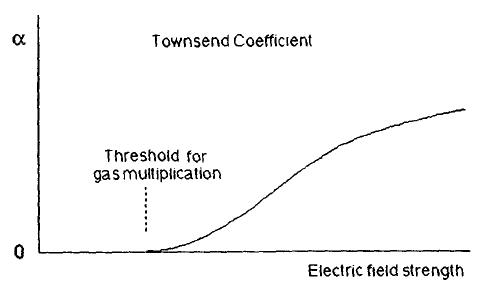
\includegraphics[width=.5\linewidth]{townsend_coefficient}
  \caption{The first Townsend coefficient as a function of the applied field\autocite{Knoll:RadMeasurement}.}
  \label{fig:town_coeff}
\end{figure}
When a ionizing particle interacts with neutral molecules, an \emph{ion pair} is
formed. This can happen either by direct interaction with the incident radiation
or by interaction with secondary electrons that gained enough kinetic energy to
ionize the molecules.

While for a low value of the field electron-ion pair simply drift towards the
electrodes, above a certain threshold of the filed, electrons rapidly gain
kinetic energy and if it is greater than the ionization energy of the neutral
gas molecules an additional ion pair is created. The electrons liberated in such
a way, will also gain kinetic energy and, colliding with the neutral gas
molecules, produce additional ionization. This \emph{gas multiplication} process
in which each electron may ionize a neutral gas molecule is known as
\emph{Townsend avalache}, the Townsend equation
\begin{equation}
  \label{eq:townsend}
  \frac{\ud n}{n} = \alpha\, \ud x
\end{equation}
where $\alpha$ is the \emph{first Townsend coefficient}, describes the increase
of the number of electrons ($n$) per unit length ($\ud
x$). Figure~\ref{fig:town_coeff} shows the slope of the $\alpha$ coefficient,
its value is zero when the electron energy is less than the multiplication
threshold and grows with the field strength afterwards. For a cylindrical
symmetry the avalanche increases in the direction of the field, moreover, the
solution of the Townsend equation
\begin{equation}
  \label{eq:townsend_sol}
  n(x) = n(0) e^{\alpha x}
\end{equation}
tells us that the number of electrons has an exponential growth with distance,
thus the growth with distance of the avalanche is even higher.

This multiplication of the charge can give a better signal over noise ration while
diminishing the requirement for an external amplifier. The key point is that the
number of secondary ionization can be kept proportional to the number of primary
ionization but the number of ions can be multiplied by a large factor. As a last
remark, sine the high energy electron avalanche interacts with many atoms, a
variety of different atomic states is formed, thus proportional counters are
sensitive to the gas composition used.

\mbox{}

Introduce here ion saturation and regions of operation that leads to gas
multiplication.


%%% Local Variables:
%%% mode: latex
%%% TeX-master: "prop_counter"
%%% End:
